\section{Analysis Results}
\label{sec:hh_results}

\begin{table}[!htb]
    \begin{center}
        \begin{tabular}{l | c c}
        \hline
        \hline
                & \multicolumn{2}{c}{\textbf{Regions}} \\
            \cline{2-3}
            \textbf{Process} & \textbf{SR-SF} & \textbf{SR-DF} \\
            \hline
            Observed Data   & 16 & 9 \\
            \hline
            Post-fit Total SM & $14.88 \pm 2.12$ & $4.88 \pm 1.24$ \\
            \hline
            Post-fit \ttbar & $2.57 \pm 0.97$ & $1.74 \pm 0.66$ \\
            Post-fit Single-top $Wt$ & $2.27 \pm 0.54$ & $2.04 \pm 0.64$ \\
            Post-fit $Z$+heavy-flavor & $7.76 \pm 1.04$ & $0.21 \pm 0.05$ \\
            \hline
            SM & $14.12 \pm 2.05$ & $5.83 \pm 1.42$ \\
            \hline
            \ttbar & $3.26 \pm 1.17$ & $2.20 \pm 0.80$ \\
            Single-top $Wt$ & $2.88 \pm 0.59$ & $2.58 \pm 0.75$ \\
            $\ttbar + V$ & $0.59 \pm 0.07$ & $0.07  \pm 0.06$ \\
            $Z$+heavy-flavor & $5.71 \pm 0.74$ & $0.15 \pm 0.04$ \\
            $Z$+light-flavor & $0.32 \pm 0.14$ & $0.00 \pm 0.00$ \\
            Single-higgs & $0.72 \pm 0.09$ & $0.32 \pm 0.06$ \\
            Fakes & $0.54 \pm 0.38$ & $0.42 \pm 0.36$ \\
        \hline
        \hline
        \end{tabular}
    \end{center}
\end{table}


\begin{figure}[!htb]
    \begin{center}
        %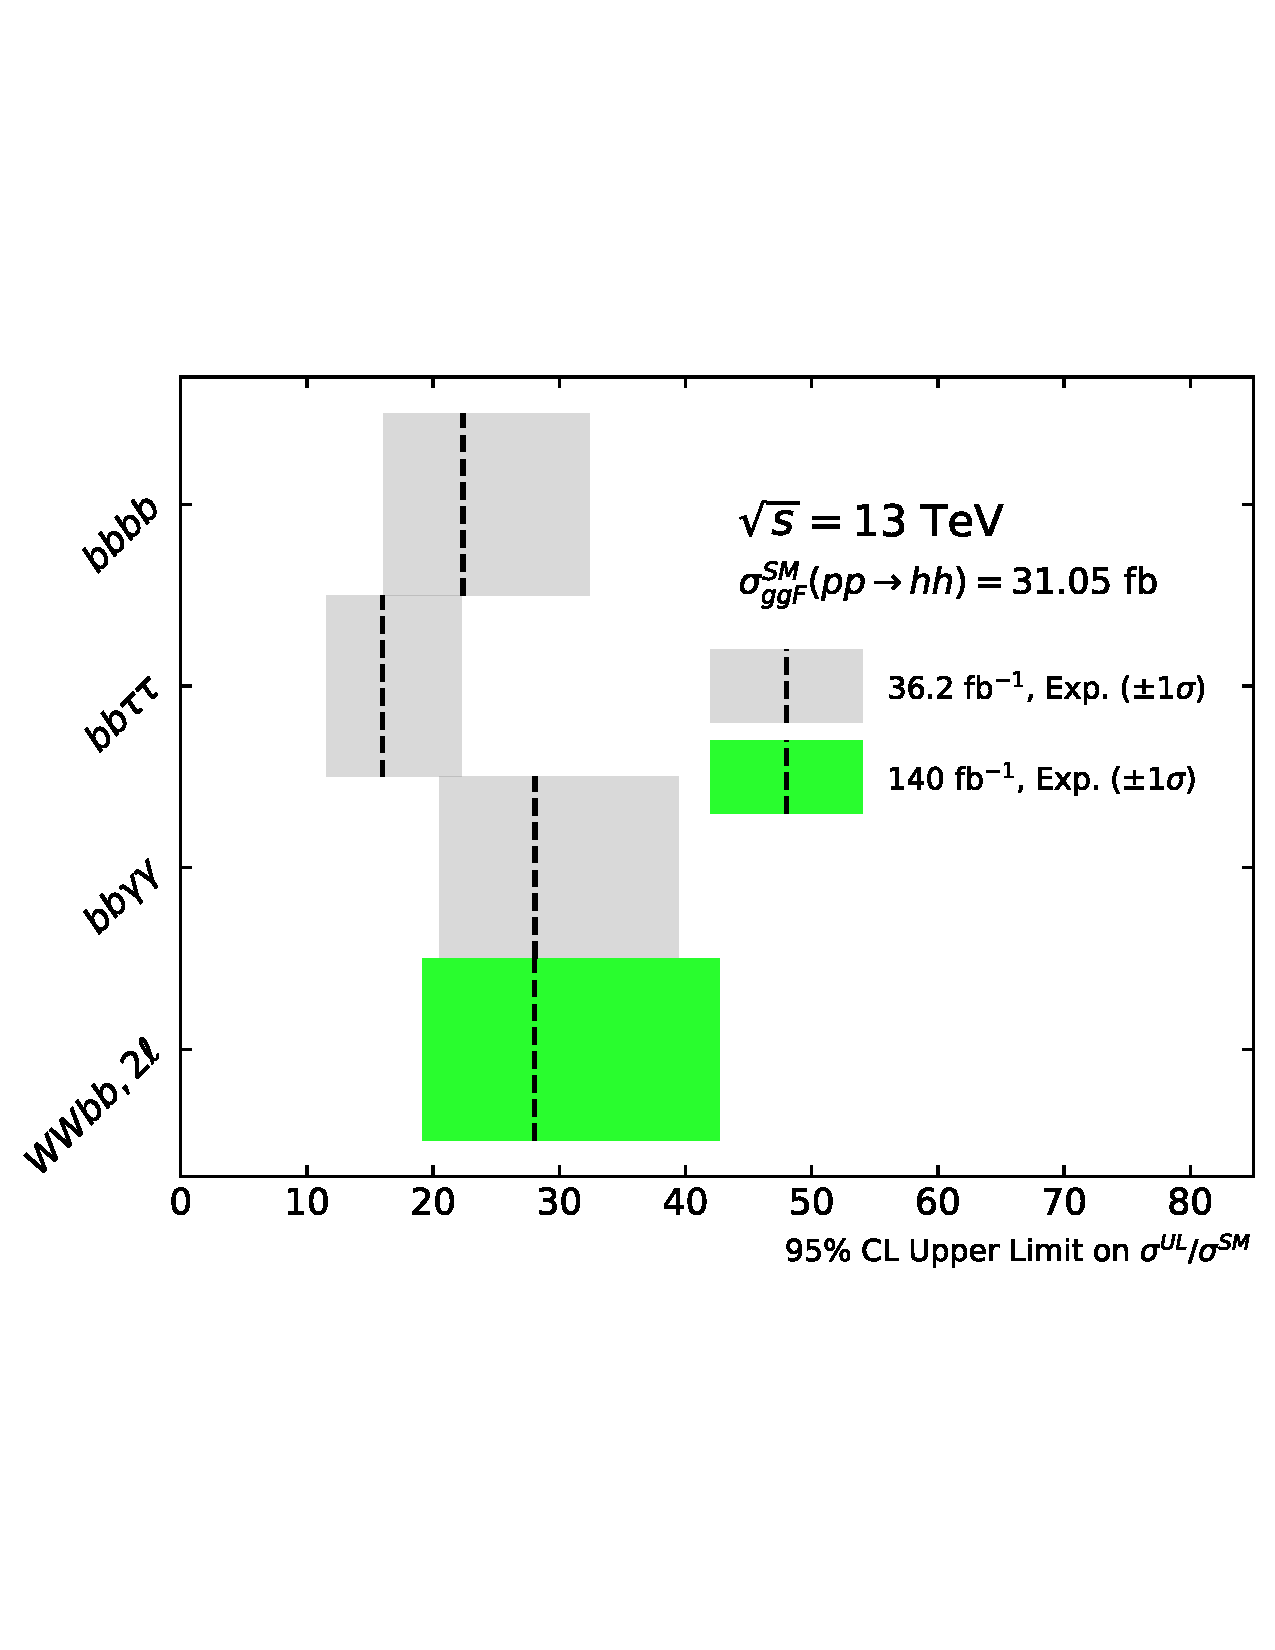
\includegraphics[width=0.75\textwidth]{figures/search_hh/results/atlas_jam_ul_plot_apr16}
        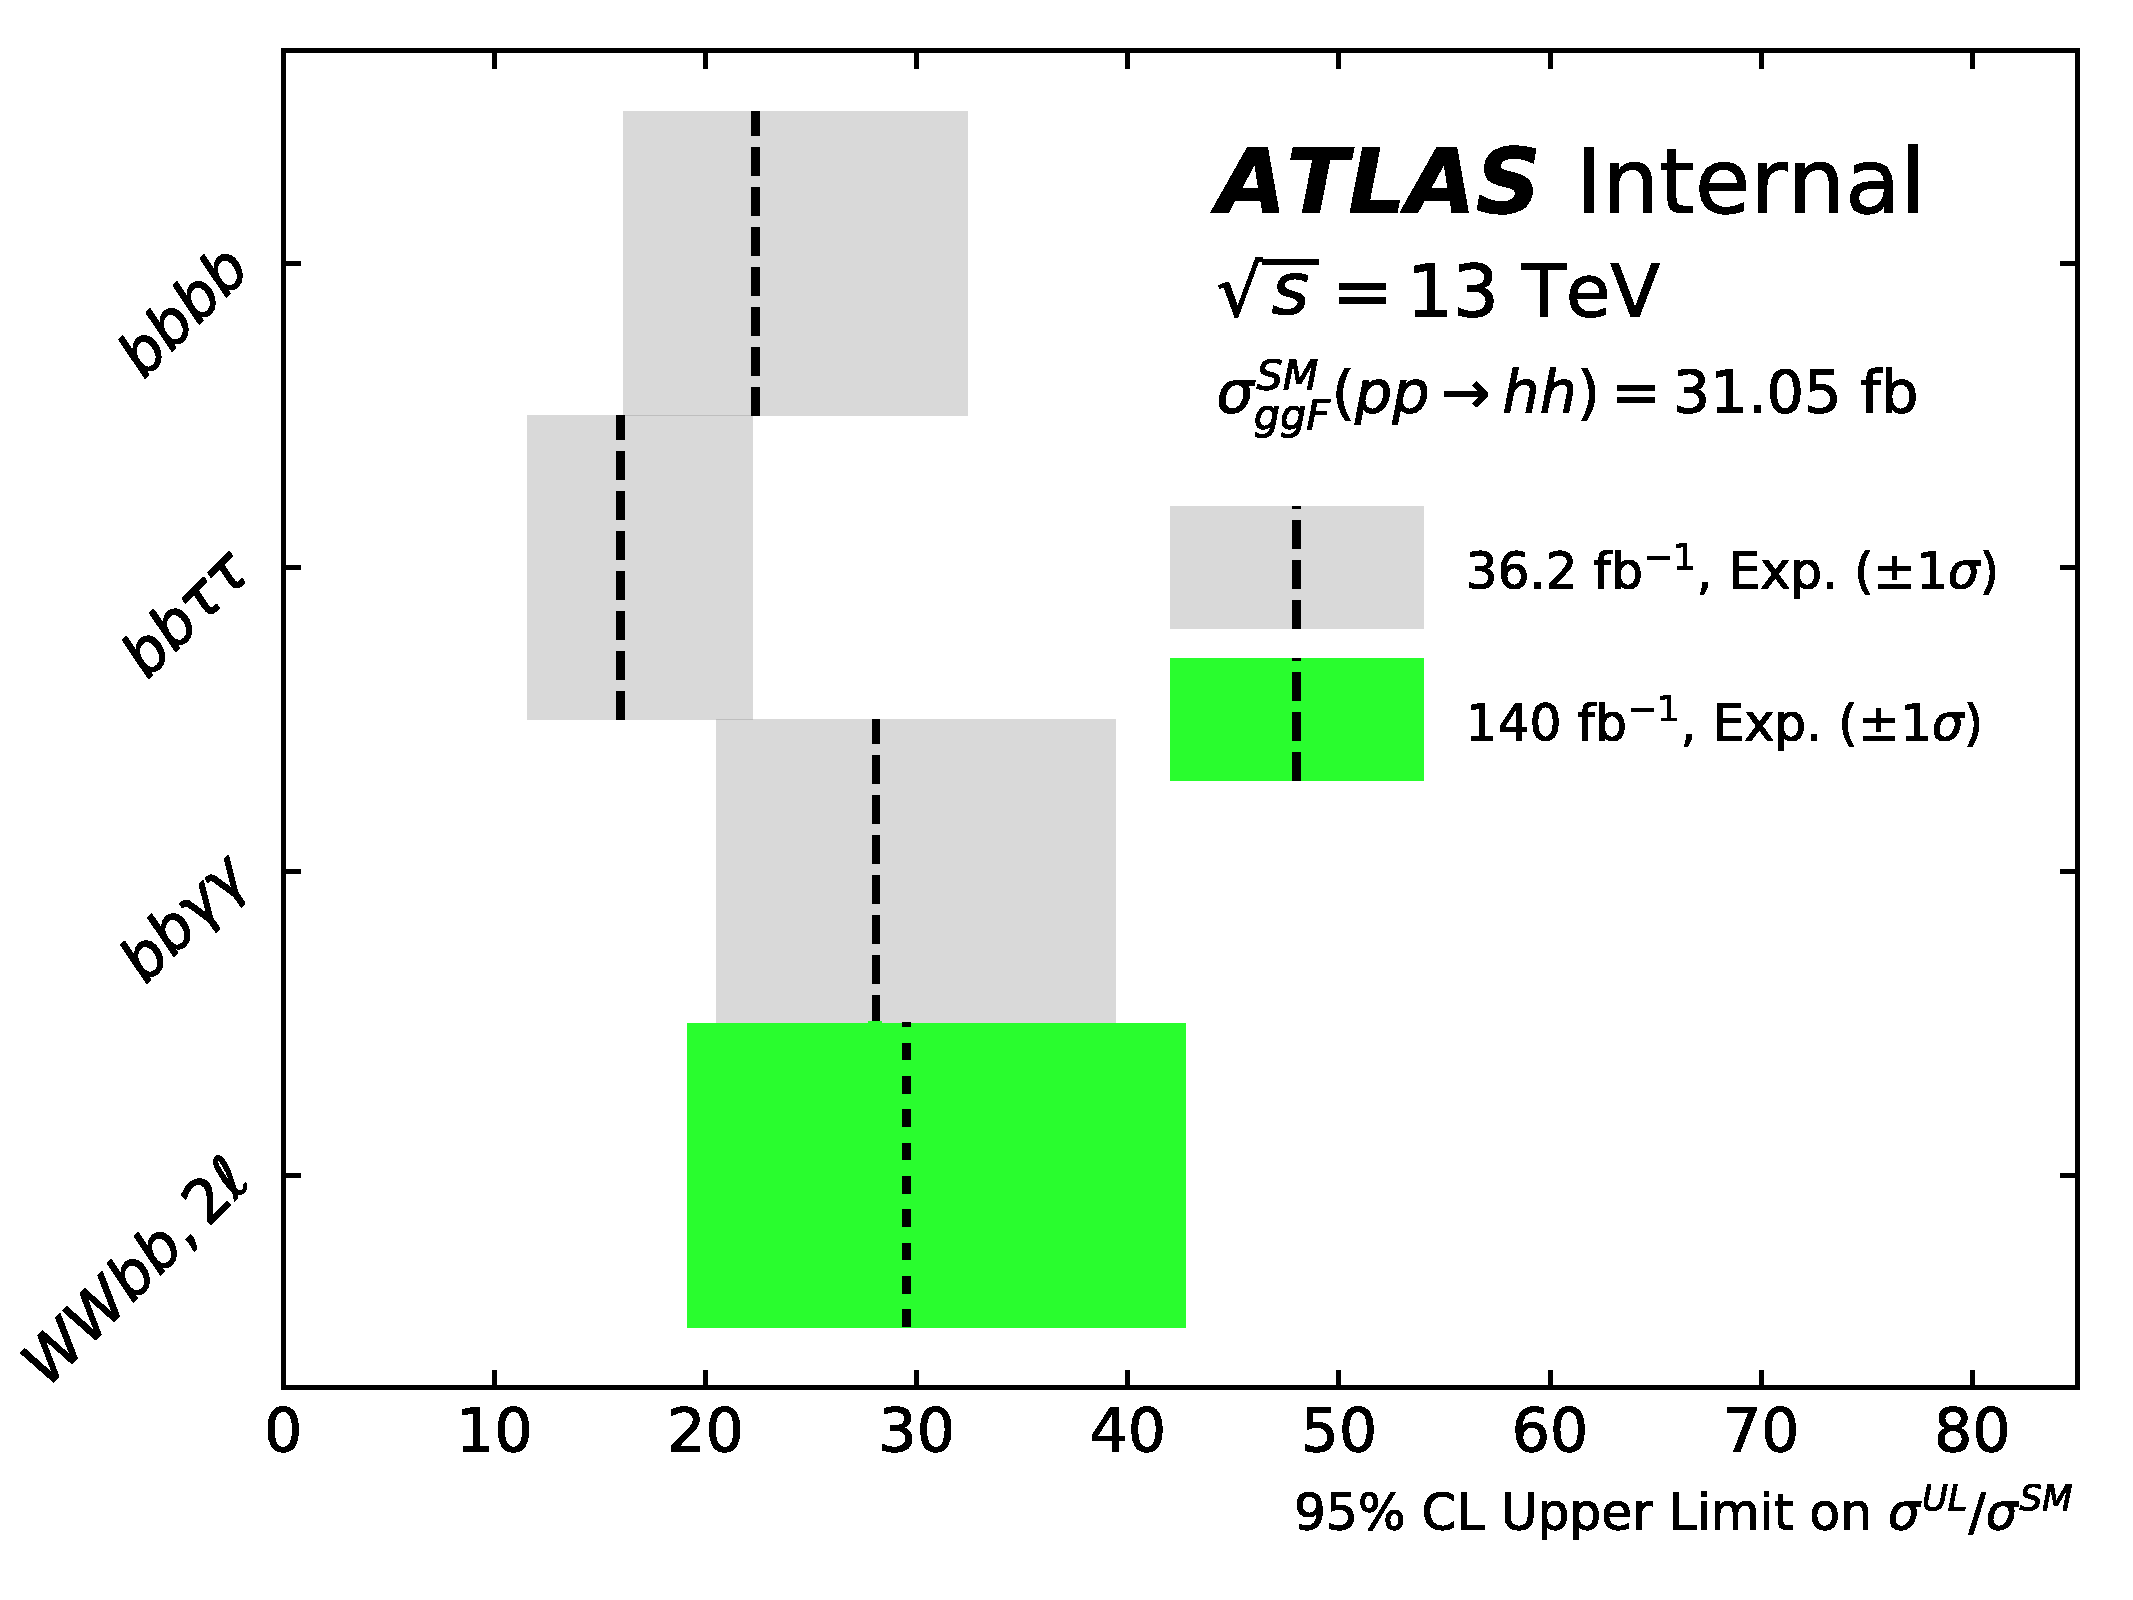
\includegraphics[width=0.75\textwidth]{figures/search_hh/results/hh_ul_compPDF}
        \caption{
            Summary plot showing the $hh$ production cross-section upper limit results, normalized to
            the SM prediction of 31.05\,fb, for the analysis presented in this thesis in green,
            based on the full Run 2 dataset of 139\,fb$^{-1}$ of $pp$ collision data.
            In grey, the partial Run 2 results based on 36\,fb$^{-1}$ of data are shown for comparison.
            Only the expected upper limits are shown.
        }
        \label{fig:hh_ul_comp}
    \end{center}
\end{figure}

\begin{figure}[!htb]
    \begin{center}
        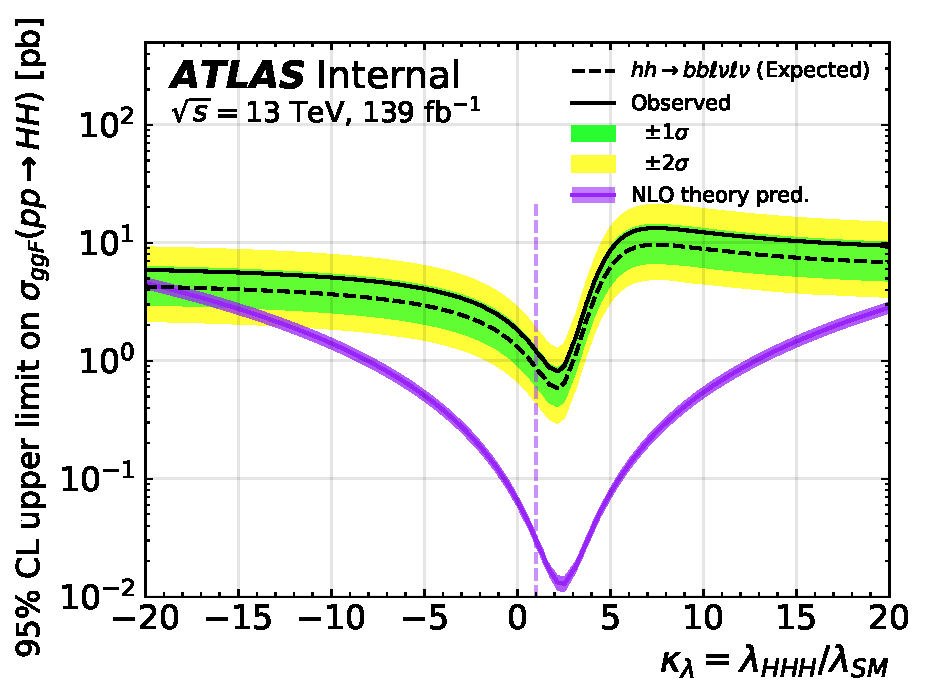
\includegraphics[width=0.75\textwidth]{figures/search_hh/results/wwbb_lambda_scan_may7}
        \caption{
            Expected and observed cross-section upper-limit for the dilepton $hh \rightarrow \bbww$ search
            as a function of the Higgs self-coupling parameter, $\kappa_{\lambda} = \lambda_{hhh} / \lambda_{hhh}^{\text{SM}}$.
            The vertical dashed line indicates the SM scenario with $\kappa_{\lambda} = 1$.
            The $\pm 1\sigma$ and $\pm 2 \sigma$ uncertainty band on the expected upper-limit includes the effects
            of all experimental and modelling systematic uncertainties.
            The NLO theory prediction is taken from Ref.~\cite{deFlorian:2016spz} and described fully
            in Ref.~\cite{HHComb36}.
        }
        \label{fig:hh_lambda_scan}
    \end{center}
\end{figure}

\begin{figure}[!htb]
    \begin{center}
        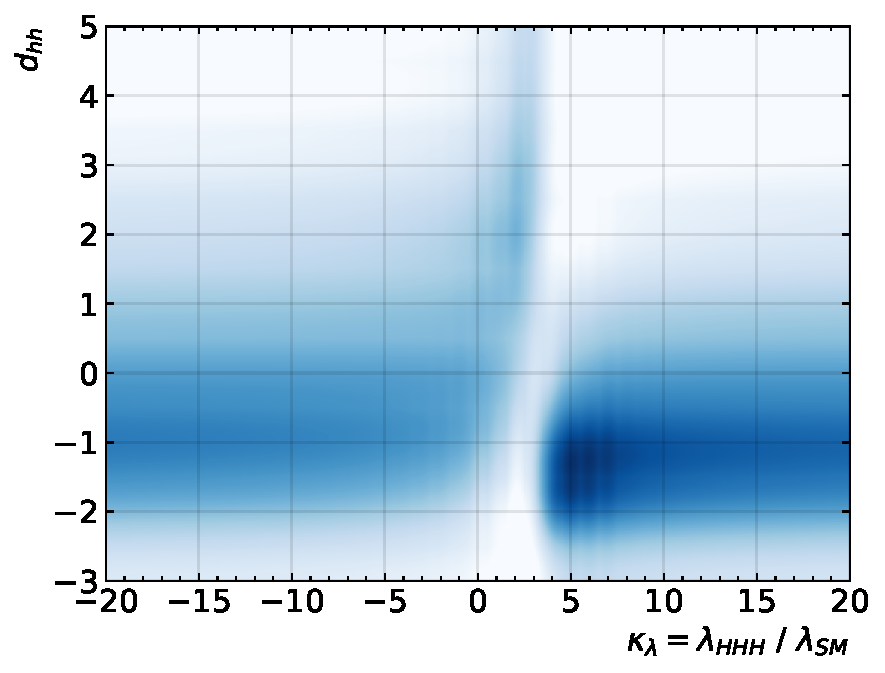
\includegraphics[width=0.75\textwidth]{figures/search_hh/results/dhh_vs_lambda}
        \caption{
            The \dhh distribution as a function of the Higgs self-coupling parameter, $\kappa_{\lambda} = \lambda_{hhh} / \lambda_{hhh}^{\text{SM}}$.
            The trend of the \dhh distribution as a function of $\kappa_{\lambda}$ is directly related to the analysis'
            acceptance to the dilepton $hh \rightarrow \bbww$ signal under non-SM values of $\kappa_{\lambda}$,
            illustrated in Figure~\ref{fig:hh_lambda_scan}.
            The darker the blue color means a higher population of the dilepton $hh \rightarrow \bbww$ signal process.
            The color white indicates that a given region is not populated at all.
        }
        \label{fig:dhh_vs_lambda}
    \end{center}
\end{figure}
